\documentclass[letterpaper]{article}
\usepackage[margin=1in]{geometry}
\usepackage[utf8]{inputenc}
\usepackage{textcomp}
\usepackage{amssymb}
\usepackage{natbib}
\usepackage{graphicx}
\usepackage{gensymb}
\usepackage{amsthm, amsmath, mathtools}
\usepackage[dvipsnames]{xcolor}
\usepackage{enumerate}
\usepackage{mdframed}
\usepackage[most]{tcolorbox}
\usepackage{csquotes}
% https://tex.stackexchange.com/questions/13506/how-to-continue-the-framed-text-box-on-multiple-pages

\tcbuselibrary{theorems}

\newcommand{\R}{\mathbb{R}}
\newcommand{\Z}{\mathbb{Z}}
\newcommand{\N}{\mathbb{N}}
\newcommand{\Q}{\mathbb{Q}}
\newcommand{\C}{\mathbb{C}}
\newcommand{\code}[1]{\texttt{#1}}
\newcommand{\mdiamond}{$\diamondsuit$}
\newcommand{\PowerSet}{\mathcal{P}}
\newcommand{\Mod}[1]{\ (\mathrm{mod}\ #1)}
\DeclareMathOperator{\lcm}{lcm}

%\newtheorem*{theorem}{Theorem}
%\newtheorem*{definition}{Definition}
%\newtheorem*{corollary}{Corollary}
%\newtheorem*{lemma}{Lemma}
\newtheorem*{proposition}{Proposition}


\newtcbtheorem[number within=section]{theorem}{Theorem}
{colback=green!5,colframe=green!35!black,fonttitle=\bfseries}{th}

\newtcbtheorem[number within=section]{definition}{Definition}
{colback=blue!5,colframe=blue!35!black,fonttitle=\bfseries}{def}

\newtcbtheorem[number within=section]{corollary}{Corollary}
{colback=yellow!5,colframe=yellow!35!black,fonttitle=\bfseries}{cor}

\newtcbtheorem[number within=section]{lemma}{Lemma}
{colback=red!5,colframe=red!35!black,fonttitle=\bfseries}{lem}

\newtcbtheorem[number within=section]{example}{Example}
{colback=white!5,colframe=white!35!black,fonttitle=\bfseries}{def}

\newtcbtheorem[number within=section]{note}{Important Note}{
        enhanced,
        sharp corners,
        attach boxed title to top left={
            xshift=-1mm,
            yshift=-5mm,
            yshifttext=-1mm
        },
        top=1.5em,
        colback=white,
        colframe=black,
        fonttitle=\bfseries,
        boxed title style={
            sharp corners,
            size=small,
            colback=red!75!black,
            colframe=red!75!black,
        } 
    }{impnote}
\usepackage[utf8]{inputenc}
\usepackage[english]{babel}
\usepackage{fancyhdr}
\usepackage[hidelinks]{hyperref}

\pagestyle{fancy}
\fancyhf{}
\rhead{CSE 100}
\chead{September 28th, 2021}
\lhead{Course Notes}
\rfoot{\thepage}

\setlength{\parindent}{0pt}

\begin{document}

\begin{titlepage}
    \begin{center}
        \vspace*{1cm}
            
        \Huge
        \textbf{CSE 100 Notes}
            
        \vspace{0.5cm}
        \LARGE
        Advanced Data Structures
            
        \vspace{1.5cm}
            
        \vfill
            
        Fall 2021\\
        Taught by Professor Niema Moshiri
    \end{center}
\end{titlepage}

\pagenumbering{gobble}

\newpage 

\pagenumbering{gobble}
\begingroup
    \renewcommand\contentsname{Table of Contents}
    \tableofcontents
\endgroup

\newpage
\pagenumbering{arabic}


% ======================================================== %
%                   NEW SECTION                            %
% ======================================================== %
\section{A Brief Introduction}
In this course, we will primarily be building off of our prior knowledge of data structures (CSE 12). In particular, we will: 
\begin{itemize}
    \item Analyze data structures for both time and space complexity. 
    \item Describe the strengths and weaknesses of a data structure. 
    \item Implement complex data structures correctly and efficiently. 
\end{itemize}


% https://www.youtube.com/watch?v=_vpy1Flh__4&list=PLM_KIlU0WoXmkV4QB1Dg8PtJaHTdWHwRS&index=2
\subsection{Data Structures vs. Abstract Data Types}
When talking about data, we often hear about data structures and abstract data types. 

\begin{center}
    \begin{tabular}{|p{7cm}|p{7cm}|}
        \hline 
        \textbf{Data Structures} (DS) & \textbf{Abstract Data Type} (ADT) \\
        \hline 
        Data structures are collections that contain: 
        \begin{itemize}
            \item Data values. 
            \item Relationships among the data. 
            \item Operations applied to the data. 
        \end{itemize}
        It also describes how the data are organized and how tasks are performed. So, a data structure defines every single detail about anything relating to the data. 
        &
        Abstract data types are defined primarily by its \underline{behavior} from the view of the \underline{user}. So, not necessarily how the operations are done, but rather what operations it must have from a completely abstract point of view.  
    
        \bigskip 
    
        Specifically, it describes only what needs to be done, not how it's done. \\
        \hline 
    \end{tabular}
\end{center}

Consider the \code{ArrayList} (DS) vs. the \code{List} (ADT).
\begin{itemize}
    \item A \code{List} will most likely have the following operations: 
    \begin{itemize}
        \item \code{add}: Adds an element to the list.
        \item \code{find}: Does an element exist in the list? 
        \item \code{remove}: Remove an element from the list. 
        \item \code{size}: How many elements are in this list? 
        \item \code{ordered}: Each element should be ordered in the way we added it. For example, if we added \code{5}, and \emph{then} added \code{3}, and \emph{then} added \code{10}, our list should look like: \code{[5, 3, 10]}.   
    \end{itemize}

    Of course, as an abstract data type, \code{List} isn't going to define how these operations work. It just lists all operations that any implementing data structure must have. In other words, we can think of \code{List}, or any abstract data type, as a \emph{blueprint} for future data structures. 

    \item An \code{ArrayList} is simply an array that is expandable. It is internally backed by an \underline{array}. So, we can perform the following operations: 
    \begin{itemize}
        \item We can \code{add} an element to the \code{ArrayList}. In this case, we add the element to the next available slot in the array, expanding the array if necessary. 
        \item We can \code{find} an element in the \code{ArrayList}. In this case, we can search through each slot of the array until we find the array or we reach the end of the array.
        \item We can \code{remove} an element from the \code{ArrayList}. In this case, we can simply move every element after the specified element back one slot. 
        \item We can get the \code{size} of the \code{ArrayList}. In this case, this is as simple as seeing how many elements are in this \code{ArrayList}.
        \item And, we know that the \code{ArrayList} is \code{ordered}. In this case, this is already done via the \code{add} and \code{remove} methods.  
    \end{itemize}
    Notice how \code{ArrayList} specifies how each operation defined by \code{List} works. In this sense, we say that \code{ArrayList} essentially implements \code{List} because we need to define \emph{how} the tasks defined by \code{List} are performed. 
\end{itemize}
So, the key takeaways are: 
\begin{itemize}
    \item An abstract data type (in our case, \code{List}) specifies what needs to be done without specifying how it's done. 
    \item A data structure (in our case, \code{ArrayList}) actually defines \textbf{how} the data is organized, how the different operations are performed, and how exactly everything is represented.
\end{itemize}











% ======================================================== %
%                   NEW SECTION                            %
% ======================================================== %
\newpage 
\section{Introduction to C++}
Here, we will talk about C++, the programming language that we will use in this course. 

% https://www.youtube.com/watch?v=8FGvlugzS5A&list=PLM_KIlU0WoXmkV4QB1Dg8PtJaHTdWHwRS&index=4
\subsection{Data Types}
First, we'll compare the data types in Java and C++. 
\begin{center}
    \begin{tabular}{|c|c|c|}
        \hline 
        \textbf{Data Type} & \textbf{Java} & \textbf{C++} \\ 
        \hline 
        \code{byte} & 1 byte & 1 byte \\ 
        \code{short} & 2 bytes & 2 bytes \\ 
        \code{int} & 4 bytes & 4 bytes \\ 
        \code{long} & 8 bytes & 8 bytes \\ 
        \code{long long} & & 16 bytes \\ 
        \hline 
        \code{float} & 4 bytes & \code{4 bytes} \\ 
        \code{double} & 8 bytes & \code{8 bytes} \\ 
        \hline 
        \code{boolean} & Usually 1 byte & \\ 
        \code{bool} &  & Usually 1 byte \\ 
        \code{char} & 2 bytes & 1 byte \\ 
        \hline 
    \end{tabular}
\end{center}
It should be mentioned that: 
\begin{itemize}
    \item In Java, you can only have signed data types. 
    \item In C++, you can have both signed and unsigned data types. 
    \item \code{boolean} (Java) and \code{bool} (C++) are effectively the same thing: they represent either \code{true} or \code{false}. 
\end{itemize}

\subsection{Strings}
There are some major differences between strings in Java and C++, which we will discuss below.

\subsubsection{Representation}
In Java, strings are represented by the \code{String} class. In C++, strings are represented by the \code{string} type.

\subsubsection{Mutability}
Strings in Java are \underline{immutable}. The moment you create a string, you won't be able to modify them. The only way to change a string variable is by creating a new string and reassigning them. 

\bigskip 

In C++, strings are actually \underline{mutable}. You can modify strings in-place. 

\subsubsection{Concatenation}
In Java, you can concatenate any type to a string. For example, the following is valid:
\begin{verbatim}
    String a = "this is a string" + 123;\end{verbatim}

In C++, you can only concatenate strings with other strings. So, if you wanted to convert an integer (or any other type) to a string, you would have to \emph{first} convert that integer to a string (or use a string stream).

\subsubsection{Substring Method}
In Java, we can take the substring of a string using the \code{substring} method. The method signature is:
\begin{verbatim}
    String#substring(beginIndex, endIndex);\end{verbatim}

In C++, we can take the substring using the \code{substr} method. The method signature is:
\begin{verbatim}
    string#substr(beginIndex, length);\end{verbatim}

An important distinction to make here is that Java's \code{substring} method takes in an \textbf{end index} for the second parameter, whereas C++'s \code{substr} method takes in a \textbf{length} for the second parameter.



\subsection{Comparing Non-Primitive Objects}
Suppose \code{a} and \code{b} are two non-primitive objects.

\bigskip 

In Java, if we want to compare these two objects, we have to make use of the methods: 
\begin{verbatim}
    a.equals(b)
    a.compareTo(b)
\end{verbatim}
If we tried using the relational operators like \code{==} or \code{!=}, Java would compare the memory addresses of the two objects, which is often something that we aren't looking for.

\bigskip 

In C++, even if \code{a} and \code{b} are objects, we can make use of the relational operators:
\begin{verbatim}
    a == b      a != b
    a < b       a <= b
    a > b       a >= b
\end{verbatim}
This is done through something called \textbf{operator overloading}, where we write a custom class and define how these operators should function.


\subsection{Variables}
Now, we will briefly discuss how variables function in both C++ and Java. 

\subsubsection{Initialization}
In Java, variable initialization is \textbf{checked}. Consider the following code: 
\begin{verbatim}
    int fast;
    int furious; 
    int fastFurious = fast + furious;
\end{verbatim}
Because \code{fast} and \code{furious} aren't initialized, the Java compiler will throw a compilation error. 

\bigskip 

In C++, variable initialization is \textbf{not checked}. Consider the same code, which will compile:
\begin{verbatim}
    int fast;
    int furious; 
    int fastFurious = fast + furious;
\end{verbatim}
Here, this would result in \textbf{undefined} behavior.

\subsubsection{Narrowing}
In Java, if we have a higher variable type and then try to cast this type to a smaller type, we would get a compilation error. Consider the following code:
\begin{verbatim}
    int x = 40_000;
    short y = x;
\end{verbatim}
This code would result in a compilation error. If we didn't want a compilation error, we would have to explicitly \emph{cast} the bigger variable type to the smaller type. The following Java code would compile just fine: 
\begin{verbatim}
    int x = 40_000;
    short y = (short) x;
\end{verbatim}

\bigskip 

In C++, no compilation error would occur; that is, the following code would compile:
\begin{verbatim}
    int x = 40_000;
    short y = x;
\end{verbatim}
What would actually happen is that \code{x} would get \textbf{truncated} when it is assigned to \code{y}, resulting in integer overflow. 


\subsubsection{Variable Declaration}
In Java, variables \textbf{cannot} be declared outside of a class. The following Java code would result in a compile error:
\begin{verbatim}
    // MyClass.java 

    int meaningOfLife = 42;
    class MyClass {
        // some code 
    }
\end{verbatim}
In order for this to compile, you have to put variable declarations inside the class space (as an instance variable) or in a method inside a class (as a local variable). 

\bigskip 

In C++, variables \textbf{can} be declared outside of a class. The following C++ code would compile completely fine: 
\begin{verbatim}
    // MyClass.cpp

    int meaningOfLife = 42;
    class MyClass {
        // some code 
    }
\end{verbatim}
Here, \code{meaningOfLife} is a \textbf{global variable}. Anything in this file can access this variable. In general, it is considered poor practice to use global variables except in cases of constants. 

\subsection{Classes, Source Code, and Headers}
Another thing that is important is the concept of classes (which leads to the topic of object-oriented programming). That being said, Java and C++ has some differences with regards to how classes function. 

\subsubsection{Class Declaration}
There are some key differences in how methods and instance variables are laid out in Java and C++. 

In Java, a typical class would look like: 
\begin{verbatim}
    class Student {
        public static int numStudents = 0;
        private String name; 
        
        public Student(String n) { /* Code */ }

        public void setName(String n) { /* Code */ }
        public String getName() { /* Code */ }
    }
\end{verbatim}

And in C++, a typical class would look like: 
\begin{verbatim}
    class Student {
        public: 
            static int numStudents; 

            Student(string n);
            
            void setName(string n);
            string getName() const; 

        private: 
            string name; 
    }

    int Student::numStudents = 0;
    Student::Student(string n) { /* Code */ }
    void Student::setName(string n) { /* Code */ }
    string Student::getName() const { /* Code */ }
\end{verbatim}

There are several notable differences: 
\begin{itemize}
    \item \textbf{Modifiers:} In Java, if you want your method or instance variable to have an access modifier, you explicitly state the access modifier. In C++, you have a region for your access modifier. That is, there is a \code{public} region, \code{private} region, etc. Any methods or instance variables listed under these regions will take on that access modifier. For instance, \code{setName} is in the \code{public} region, so \code{setName} is public.
    \item \textbf{Implementation:} In Java, directly after declaring a method or constructor in a class, we need to provide the implementation code. In C++, we can ``declare'' the methods and the constructor, and then outside of the class we can implement the methods.
\end{itemize}
Now, consider the following C++ code: 
\begin{verbatim}
    class Point {
        private: 
            int x; 
            int y;
        
        public:
            Point(int i, int j);
    }

    Point::Point(int i, int j) {
        x = i;
        y = j;
    }
\end{verbatim}
Here, we're initializing the \code{x} and \code{y} instance variables directly from the constructor implementation. However, we can initialize these instance variables directly like so: 
\begin{verbatim}
    class Point {
        private: 
            int x; 
            int y;
        
        public:
            Point(int i, int j);
    }

    Point::Point(int i, int j) : x(i), y(j) {}
\end{verbatim}
This is called the \textbf{member initializer list}.

\subsubsection{Source vs. Header Files}
Consider the following class: 
\begin{verbatim}
    class Student {
        public: 
            static int numStudents;
            Student(string n);
        
        private: 
            string name; 
    }

    int Student::numStudents = 0;
    Student::Student(string n) : name(n) {
        numStudents++;
    }
\end{verbatim}
We can choose to break this up into two separate files; a \textbf{source} (usually \code{.cpp}) file and a \textbf{header} (usually \code{.h}) file. The header file contains the class and the method \emph{declaration}; the source file contains the implementations for those methods. So, the above code can be written like so: 
\begin{verbatim}
    // The header file 
    // Student.h
    class Student {
        public: 
            static int numStudents;
            Student(string n);
        
        private: 
            string name; 
    }

    // The source file 
    // Student.cpp 
    int Student::numStudents = 0;
    Student::Student(string n) : name(n) {
        numStudents++;
    }
\end{verbatim}

\subsection{Memory Diagrams}
Consider the following Java code: 
\begin{verbatim}
    Student s1 = new Student("Niema");
    Student s2 = s1;
\end{verbatim}
Here, \code{s1} is a \emph{reference} to a \code{Student} object. This \code{Student} object contains a \emph{reference} to a \code{string} object with the content \code{Niema}. That is: 
\begin{verbatim}
    Student object
    |----------|
    | |----|   |   (Reference)  |-------|
    | |name|------------------> | Niema |
    | |----|   |                |-------|
    |----------|   <------      String object
       /|\                \
        |                  \
        |                   \ (Reference)
        |                   |
        | (Reference)       |
    s1 -/                   s2
\end{verbatim} 
It also follows that \code{s2} is a reference to the same object that \code{s1} is referring to. 

\bigskip 

Now, consider the following C++ code: 
\begin{verbatim}
    Student s1("Niema");
    Student s2 = s1;
\end{verbatim}
Here, \code{s1} is a \code{Student} \emph{object}. The \code{Student} object contains a \code{string} object with the content \code{Niema}. That is:
\begin{verbatim}
    |-----------------|     |-----------------|
    | |-----------|   |     | |-----------|   |
    | |name: Niema|   |     | |name: Niema|   |
    | |-----------|   |     | |-----------|   |
    |  string object  |     |  string object  |
    |-----------------|     |-----------------|
    Student object          Student object
       s1                       s2
\end{verbatim} 
Additionally, when we assign \code{s1} to \code{s2}, we actually make a copy of said object. So, \code{s2} is its own object; it does not share a reference with \code{s1}.

\bigskip 

In other words, in Java, \code{s1} and \code{s2} are both references to the same object; in C++, \code{s1} \emph{is} the object and \code{s2} is \emph{another} object.

\subsubsection{References}
Consider the following C++ code: 
\begin{verbatim}
    Student s1 = Student("Niema");
    Student & s2 = s1;
    Student s3 = s2;
\end{verbatim}
The memory diagram looks like this: 
\begin{verbatim}
    |-----------------|     |-----------------|
    | |-----------|   |     | |-----------|   |
    | |name: Niema|   |     | |name: Niema|   |
    | |-----------|   |     | |-----------|   |
    |  string object  |     |  string object  |
    |-----------------|     |-----------------|
    Student object          Student object 
       s1      s2               s3
\end{verbatim} 
Here, \code{s2} can be seen as \emph{another} way to call \code{s1} (think of \code{s2} as another name for \code{s1}). \code{s3} would be a copy of \code{s1}. 

\subsubsection{Pointers}
Pointers are similar to Java references. Consider the following C++ code: 
\begin{verbatim}
    Student s = Student("Niema");
    // * in this case means pointer 
    // & means memory address
    // So, ptr stores a memory address to some object. In other words, 
    // it points to the object s. 
    Student* ptr = &s; 
    Student** ptrPtr = &ptr; 
\end{verbatim}
The memory diagram would look like: 
\begin{verbatim}
    Mem. Address: 9500 
    |-----------------|
    | |-----------|   |       |-----------|       |-----------|
    | |name: Niema|   |  <--- |    9500   |  <--- |           |
    | |-----------|   |       |-----------|       |-----------|
    |  string object  |       Student* (pointer)   Student** (pointer to pointer) 
    |-----------------|           ptr                  ptrPtr
    Student object      
       s
\end{verbatim} 
If we wanted to access an object through a pointer, we can do this in several ways. 
\begin{enumerate}
    \item Deferencing a pointer. 
    \begin{verbatim}
        // * in this case dereferences the pointer
        // Think of the * as following the arrow  
        (*ptr).name; 
    \end{verbatim}

    \item Arrow dereferencing. 
    \begin{verbatim}
        // ptr->x is the same thing as (*ptr).x
        ptr->name; 
    \end{verbatim}
\end{enumerate}

\subsubsection{Memory Management}
Consider the following C++ code: 
\begin{verbatim}
    Student s1 = Student("Niema");
    Student* s2 = new Student("Ryan");
\end{verbatim}
The corresponding memory diagram is: 
\begin{verbatim}
    |-----------------|     |-----------------|
    | |-----------|   |     | |-----------|   |
    | |name: Niema|   |     | |name: Ryan |   |
    | |-----------|   |     | |-----------|   |
    |  string object  |     |  string object  |
    |-----------------|     |-----------------|
    Student object          Student object 
       s1                                 /|\
                                           |
                                           |
                                           |
                                |------|   |
                                |      | --/
                                |------|
                                Student* (pointer)
                                s2
\end{verbatim}
Here, \code{s1} is allocated on the \emph{stack}; once the method returns, \code{s1} is automatically destroyed. 

\bigskip 

\code{s2} is allocated through the \code{new} keyword. This is known as dynamic memory allocation. So, \code{s2} is a pointer to the newly allocated memory. Because this object was created using the \code{new} keyword, we need to deallocate it ourselves. To do so, we need to explicitly call \code{delete} on this object: 
\begin{verbatim}
    delete s2; 
\end{verbatim}
\code{delete} takes in a memory address (i.e. pointer). This is very similar to \code{free} (in C). If we don't free this, we run into what is called a \textbf{memory leak}. 

\subsection{Constant Keyword}
In C++, the \code{const} keyword means that the variable can never be reassigned. Consider the following: 
\begin{verbatim}
    const int a = 42; 
    int const b = 42;
\end{verbatim}
If we tried reassigning \code{a} (e.g. \code{a = 41;}), we would get a compiler error. 

\bigskip

The second line (\code{int const}) is identical to the first line. 


\subsubsection{\code{const} and Pointers}
Consider the following C++ code: 
\begin{verbatim}
    int a = 42;                     // a 
    const int* ptr1 = &a;           // b
    int const* ptr2 = &a;           // c
    int* const ptr3 = &a;           // d
    const int* const ptr4 = &a;     // e
\end{verbatim}
\begin{itemize}
    \item For lines (b) and (c), the pointer cannot modify the object that it is pointing to.  But, we can reassign the pointer to point to a different object. 
    \item For line (d), we cannot reassign the pointer to point to a different object. However, we can modify the object that the pointer is pointing to. 
    \item For (e), we cannot reassign the pointer to point to a different object \emph{or} modify the object that the pointer is pointing to. 
\end{itemize}
In general:
\begin{verbatim}
    const type* const varName = ...; 
    ----------- -------------
       (a)            (b)
\end{verbatim}
\begin{itemize}
    \item Segment (A): The \code{const} next to \code{type*} means that we cannot modify the object or value behind the pointer. 
    \item Segment (B): The \code{const} next to \code{varName} (the variable name) means that we cannot reassign the pointer to point to a different object or value. 
\end{itemize}

\subsubsection{\code{const} and References}
Suppose we have the following C++ code: 
\begin{verbatim}
    int a = 42; 
    const int & ref1 = a;       // a
    int const & ref2 = a;       // b
\end{verbatim}
\begin{itemize}
    \item In (a), the \code{const} means that we cannot modify the variable through the constant reference. So: 
    \begin{verbatim}
        a = 21;         // Allowed. 
        ref1 = 20;      // Compile error!
    \end{verbatim}

    \item (b) is the same exact thing is (a).
\end{itemize}

\subsubsection{\code{const} Functions}
Recall the \code{Student} class from earlier: 
\begin{verbatim}
    class Student {
        public: 
            Student(string n);
            string getName() const; 
            
        private: 
            string name; 
    }

    Student::Student(string n) : name(n) {}
    string Student::getName() const {
        return name;
    }
\end{verbatim}
What does the \code{const} in \code{getName()} do? Well, the \code{const} keyword after the function declaration means that the function cannot modify \emph{this} object. So: 
\begin{itemize}
    \item You cannot do any assignments to instance variables. 
    \item You can only call other \code{const} functions.
\end{itemize} 
So, effectively, \code{const} after a function name means that we are guaranteeing that we aren't changing the object's state in any way.

\subsection{Functions}
In C++, we can have global functions (functions that are defined outside of classes). For instance, the main method (shown below) is a global function (and is required to be):
\begin{verbatim}
    int main() {
        /* Do stuff */ 
    }

    class MyClass {
        /* Some code */ 
    }
\end{verbatim}

\subsubsection{Passing by Value vs. Reference}
In C++, you can pass parameters either by value or reference. 

\bigskip

When passing by value, the function makes a \textbf{copy} of the values that you passed in. Some example code is shown below:
\begin{verbatim}
    void swap(int a, int b) {
        int tmp = a;
        a = b;
        b = tmp;
    }
\end{verbatim}
These copies are destroyed once the function returns (the stack frame is destroyed). 

\bigskip 

When passing by reference, the function takes in \emph{references} to the variables. Some example code is shown below:
\begin{verbatim}
    void swap(int & a, int & b) {
        int tmp = a;
        a = b;
        b = tmp;
    }
\end{verbatim}
Effectively, whatever you change with the references will be reflected with the actual variables. So, in the above \code{swap} method, \code{a} and \code{b} will be updated after the function is done. 

\subsection{Vectors}
A C++ \code{vector} is very similar in nature to Java's \code{ArrayList} class and arrays. Consider the following code, which demonstrates some common operations: 
\begin{verbatim}
    // Creates a new vector. 
    vector<int> a; 
    // Adds 42 to end of vector. Looks like: [42]
    a.push_back(42);
    // Adds 21 to end of vector. Looks like: [42, 21]
    a.push_back(21);
    // Removes 21 from vector. Looks like [42] 
    a.pop_back(); // returns 21 
    // We can access the first element (0th index).
    a[0];
\end{verbatim}
Like Java arrays or \code{ArrayList}, elements in a C++ vector are stored contiguously; that is, they are stored after the previous element. 

\bigskip 

We know that if we assign an object to another variable, the other variable will get a full copy of that object. The same applies to vectors; we can also create a copy of a vector simply be reassigning it:
\begin{verbatim}
    vector<int> a;
    a.push_back(42);
    vector<int> b = a;
    // a: [42]
    // b: [42]
\end{verbatim}

\subsection{Input and Output}
Consider the following code: 
\begin{verbatim}
    int n; 
    cout << "Enter a number: "; 
    cin >> n; 

    string message; 
    cout << "Enter a message: "; 
    getline(cin, message);

    if (cin.fail()) {
        cerr << "Bad input!" << endl; 
    }
\end{verbatim}
Here: 
\begin{itemize}
    \item \code{cin} represents standard input (\code{stdin}). 
    \item \code{cout} represents standard output (\code{stdout}). 
    \item \code{cerr} represents standard error (\code{stderr}).
\end{itemize}
In C++, we can use \code{istream} to handle input stream and \code{ostream} to handle output stream. \code{cin} is an example of an \code{istream}; \code{cout} is an example of an \code{ostream}. 

\bigskip 

We can make use of the overloaded \code{<<} and \code{>>} operators to write to standard output and read from standard input, respectively. So: 
\begin{itemize}
    \item \code{cout << "Enter a number"} effectively means to write this message to standard output. 
    \item \code{cin >> n} effectively means to read from the standard input and store that input into \code{n}. We aren't necessarily restricted to \code{int}; we could use \code{long}, \code{double}, \code{string}, etc. 
    \item We can also use \code{getline} to read from standard input and then store the result into a variable. In our example above, we called \code{getline(cin, message)}. \code{cin} is where we are reading the input from and \code{message} is the variable where we store the result of reading from \code{cin}. 
    \item \code{endl} means \code{end} \code{l}ine and, in our use case here, writes a new line to standard error. In reality, we can use \code{endl} to write a newline to standard output or error.  
\end{itemize}

\subsection{Templates}
Templates introduce the notion of \emph{generic programming}. Consider the following code in Java: 
\begin{verbatim}
    class Node<Data> {
        public final Data data; 
        public Node(Data d) {
            data = d;
        }
    }

    Node<String> a = new Node<String>(s);
    Node<Integer> a = new Node<Integer>(s);
\end{verbatim}
The generic type is \code{Data} (though you can rename it to whatever you want). We can use this type either as a parameter type or a return type. When creating a new object with a generic type, we simply put the type between the \code{<>} (like with the \code{Node} examples).

\bigskip 

Consider the equivalent C++ example: 
\begin{verbatim}
    template<typename Data>
    class Node {
        public: 
            Data const data; 
            Node(const Data & d) : data(d) {}
    }

    Node<string> a(s);
    Node<int> b(n);
\end{verbatim}
Here, we can use templates to achieve similar results (compared to the Java example). Functionality-wise, this is similar to Java. 

\subsection{Iterators}
Consider the following C++ code: 
\begin{verbatim}
    for (string name : names) {
        cout << name << endl; 
    }
\end{verbatim}
What is \code{names}? 
\begin{itemize}
    \item Is it a \code{vector}? 
    \item Is it a \code{set}? 
    \item Is it an \code{unordered\_set}?
    \item Is it another collection that C++ has? 
\end{itemize}
Well, it doesn't matter! Regardless of what collection we are using, how we use it doesn't matter when it comes to iterating over it. This functionality is made possible by something called \textbf{iterators}.

\subsubsection{Iterating Over Arrays}
Consider the following code: 
\begin{verbatim}
    void printInorder(int* p, int size) {
        for (int i = 0; i < size; ++i) {
            cout << *p << endl; 
            ++p; 
        }
    }
\end{verbatim}
The \code{*p} deferences the pointer, giving the value at the location that the pointer is pointing to. 

\bigskip

The \code{++p} is an example of pointer arithmetic; this will add whatever the size of the type is to the pointer. In this case, this will make the pointer point to the memory address of the next element in the array. 

\bigskip 

Here, we know that \code{p} is (initially) a pointer to the first element in the array: 
\begin{verbatim}
     0   4   8   12  16  20  24  28         Memory Address 
     ------------------------------         (sizeof(int) = 4)
    [10, 20, 25, 30, 46, 50, 55, 60]        Array 
     ^
     p                                      Pointer 
\end{verbatim}
Dereferencing \code{p} (\code{*p}) gives us \code{10}. 

\bigskip 

When we do \code{++p}, we made the pointer point to the next memory address: 
\begin{verbatim}
    0   4   8   12  16  20  24  28         Memory Address 
    ------------------------------
   [10, 20, 25, 30, 46, 50, 55, 60]        Array 
        ^
        p                                  Pointer 
\end{verbatim}
Dereferencing \code{p} (\code{*p}) gives us \code{20}. 


\subsubsection{Using Iterators}
Consider the following C++ code: 
\begin{verbatim}
    vector<string> names; 
    // populate with data 

    vector<string>::iterator itr = names.begin(); 
    vector<string>::iterator end = names.end(); 
    
    while (itr != end) {
        cout << *itr << endl; 
        ++itr; 
    }
\end{verbatim}
Here, we note a few things. 
\begin{itemize}
    \item \code{iterator} is simply a class that handles, well, iteration. So, \code{itr} and \code{end} are instances of the \code{iterator} class that is iterating over \code{names}. 
    \item The \code{!=} operator (in \code{itr != end}) has been overloaded. This checks the \code{curr} property in the \code{iterator} class to see if it is equal (or, more specifically, not equal) to the \code{curr} property of the other index. In this case, \code{itr != end} is effectively comparing \code{itr.curr} with \code{itr.end}. 
    \item The \code{*} dereferencing operator (in \code{*itr}) has also been overloaded. This operator has been overloaded to return whatever the value is at the \code{curr} index. So, in our case,\code{*itr} would return whatever value is at the specified \code{curr} index in the array that we are iterating through. 
    \item The \code{++} operator (in \code{++itr}) is also overloaded. This will increment the \code{curr} property in the \code{iterator} instance. 
\end{itemize}

Suppose \code{names} has the following: 
\begin{verbatim}
        0       1       2           // Index 
    ["Niema", "Ryan", "Felix"]      // names array 
\end{verbatim}

Essentially, \code{vector<string>::iterator} will look something like: 
\begin{verbatim}
    |-----------------------------| |-----------------------------|
    |         |----|              | |         |----|              |
    |   curr: | 0  |              | |   curr: | 3  |              |
    |         |----|              | |         |----|              |
    |           int               | |           int               |
    |-----------------------------| |-----------------------------|
                itr                             end
\end{verbatim}
Calling \code{*itr} will basically give us \code{names[curr]} (or, more specifically, \code{names[0]}). Comparing \code{itr != end} is basically the same as checking \code{0 != 3}. 

\bigskip 

When we call \code{++itr}, we now have: 
\begin{verbatim}
    |-----------------------------| |-----------------------------|
    |         |----|              | |         |----|              |
    |   curr: | 1  |              | |   curr: | 3  |              |
    |         |----|              | |         |----|              |
    |           int               | |           int               |
    |-----------------------------| |-----------------------------|
                itr                             end
\end{verbatim}
Calling \code{*itr} now will basically give us \code{names[curr]} (or, more specifically, \code{names[1]}). Comparing \code{itr != end} is basically the same as checking \code{1 != 3}. 

\subsubsection{Linked List Iterator}
Consider the following code, which is essentially the same code as the previous one: 
\begin{verbatim}
    LinkedList<string> names; 
    // populate with data 

    LinkedList<string>::iterator itr = names.begin(); 
    LinkedList<string>::iterator end = names.end(); 
    
    while (itr != end) {
        cout << *itr << endl; 
        ++itr; 
    }
\end{verbatim}
The only difference is that we're now using a \code{LinkedList} instead of \code{vector}. However, the way the data is structured is very different. Suppose \code{names} has the following: 
\begin{verbatim}
    |---------------|      |---------------|      |---------------|
    | data: "Niema" |      | data: "Ryan"  |      | data: "Felix" |
    |     next: [ ] ---->  |     next: [ ] ---->  |     next: [x] |
    |---------------|      |---------------|      |---------------|
\end{verbatim}

Here, \code{[x]} (in the \code{next} property of the last node) is a \code{nullptr}. 

\bigskip

How does using nodes change our iterator? Well, \code{LinkedList<string>::iterator} will look something like: 
\begin{verbatim}
    |---------------|      |---------------|      |---------------|
    | data: "Niema" |      | data: "Ryan"  |      | data: "Felix" |
    |     next: [ ] ---->  |     next: [ ] ---->  |     next: [x] |
    |---------------|      |---------------|      |---------  /|\ |
               /|\                                             |
                |                                              |
                |                                  ------------/
                |                                 /  
                |                                /
    |-----------|-----------------| |------------|----------------|
    |         |-|--|              | |         |--|-|              |
    |   curr: |    |              | |   curr: |    |              |
    |         |----|              | |         |----|              |
    |         Node*               | |         Node*               |
    |-----------------------------| |-----------------------------|
                itr                             end
\end{verbatim}
Going back to the code: 
\begin{verbatim}
    while (itr != end) {
        cout << *itr << endl; 
        ++itr; 
    }
\end{verbatim}
It should be noted that: 
\begin{itemize}
    \item \code{!=} is once again overloaded to compare the values of the node's \code{data}. 
    \item \code{*itr} is once again overloaded to return \code{data}. It would look like: 
    \begin{verbatim}
        return curr->data;
    \end{verbatim}
    \item \code{++itr} is once again overloaded to make the iterator move to the next node. This would look like: 
    \begin{verbatim}
        curr = curr->next; 
    \end{verbatim}
\end{itemize}

\subsubsection{Creating an Iterator Class}
When creating data structures, we'll often need to create our own Iterator classes. 

\bigskip 

First, we'll talk about the operators associated with the iterator class: 
\begin{itemize}
    \item \code{==}: \code{true} if the iterators are pointing to the same item and \code{false} otherwise. 
    \item \code{!=}: \code{true} if the iterators are pointing to the different item and \code{false} otherwise. 
    \item \code{*} (dereference): Return a reference to the current data value. 
    \item \code{++} (pre- and post-increment): Move the iterator to the next item. 
\end{itemize}

And, we also need to talk about what functions are in the \underline{data structure class} so we can make use of the iterator:
\begin{itemize}
    \item \code{begin()}: Returns an iterator to the first element. 
    \item \code{end()}: Returns an iterator to the element just after the last element (not the last element, but \emph{after} the last element).  
\end{itemize}
So, in the Linked List example: 
\begin{verbatim}
    [] -> [] -> []
    ^              ^
    begin()        end()
\end{verbatim}
And in any array-based structures: 
\begin{verbatim}
    [a, b, c, d, e]
     ^              ^
     begin()        end()
\end{verbatim}


\newpage
\section{Time and Space Complexity}
One of the key things computer scientists try to do is automate competitive tasks, and of course, that requires \emph{performance}. So, that begs the question: how can we measure the performance of our program? 
\begin{itemize}
    \item How many hours does it take to run? 
    \item Minutes? 
    \item Nanoseconds? 
\end{itemize}
These are all metrics of \emph{human time}. However, a program has two aspects: 
\begin{itemize}
    \item The implementation. 
    \item The algorithm behind that program. 
\end{itemize}
While these different metrics of human time are good at measuring the actual implementation of a program, they don't do a good job describing how fast the \emph{idea}, the algorithm itself, is. For instance, running the algorithm on two different devices, both which have wildly different hardware, will result in a significant difference in how fast your algorithm runs. 

\bigskip 

That being said, we want to know how fast an algorithm is. The best way to do so is by figuring out the performance in terms of number of operations with respect to the input size $n$ (instead of the amount of time). 

\subsection{Notation of Complexity}
Consider the following notations: 
\begin{itemize}
    \item Big-$O$: Upper bound. 
    \item Big-$\Omega$: Lower bound. 
    \item Big-$\theta$: Both upper and lower bound. 
\end{itemize}
Consider the following graph: 
\begin{center}
    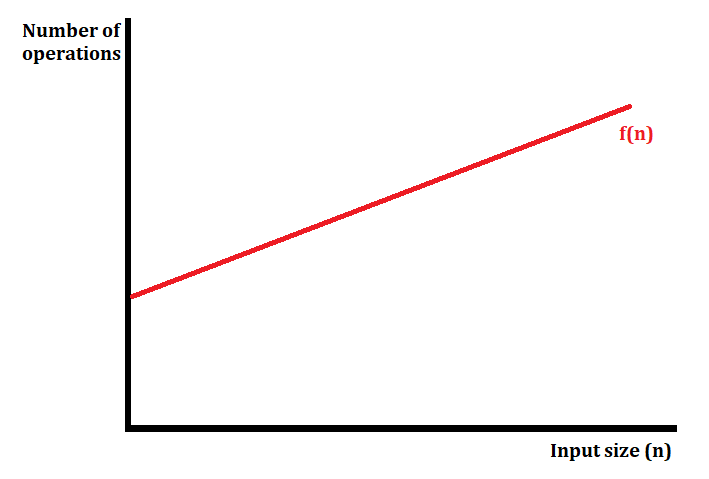
\includegraphics[scale=0.5]{img/graph1.PNG}
\end{center}
Where $f(n)$ describes the number of operations of your algorithm for some $n$. 
\begin{itemize}
    \item We say that $f(n)$ is $O(g(n))$ if, for some constant $a$, we have $a * g(n) \geq f(n)$ as $n \to \infty$. 
    
    \bigskip 

    Consider the following graph: 
    \begin{center}
        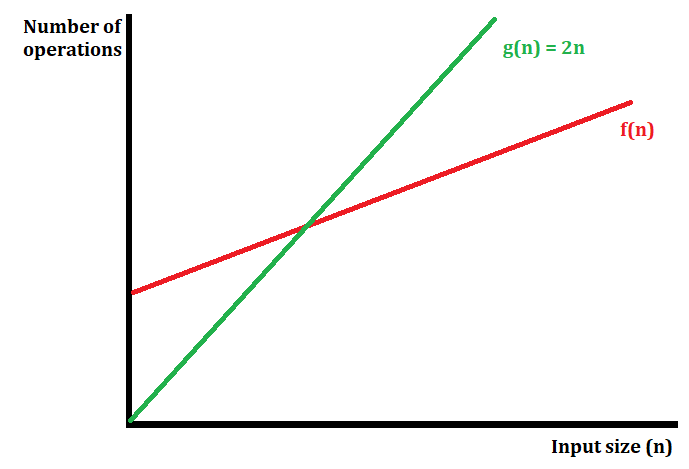
\includegraphics[scale=0.5]{img/graph2.PNG}
    \end{center}
    Here, we see that the intersection of the red and the green line occurs at some point, and that after that point the green line will always be greater than the red line. In other words, at that point, we can say that $f(n)$ will never be bigger than $g(n)$ beyond that point. Therefore, we say that $f(n)$ is $O(2n)$, or simply $O(n)$.
    
    \item Big-$\Omega$ works similarly. We say that $f(n)$ is $\Omega(g(n))$ if, for some constant $b$, $b * g(n) \leq f(n)$ as $n \to \infty$.
    
    \bigskip 

    Consider the following graph: 
    \begin{center}
        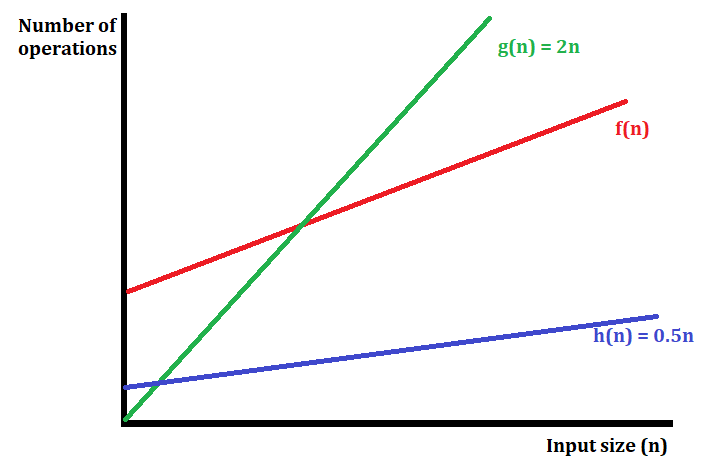
\includegraphics[scale=0.5]{img/graph3.PNG}
    \end{center}
    Here, we see that the blue line $h$ is strictly lower than the red line. In other words, $f(n)$ will never be smaller than $h(n)$. Therefore, we say that $f(n)$ is $\Omega(0.5n)$, or simply $\Omega(n)$. 
    
    \item We say that $f(n)$ is $\theta(g(n))$ if $f(n)$ is $O(g(n))$ and $f(n)$ is $\Omega(g(n))$. Mathematically: 
    \[b * g(n) \leq f(n) \leq a * g(n)\]
    
    In the graphs above, we already found the $b$ and $a$ constants. So:
    \[0.5n \leq f(n) \leq 2n\]
    Therefore, we can say $f(n)$ is $\theta(n)$.
\end{itemize}

\textbf{Remarks:} 
\begin{itemize}
    \item Your bigger or smaller functions do not need to be strictly (i.e. always) bigger or smaller than your $f(n)$. They just need to be strictly bigger or smaller beyond some $n$.
    \item We will almost always use Big-$O$. 
\end{itemize}

\subsection{Finding Big-O Time Complexity}
Given some algorithm, how do we find the Big-$O$ time complexity of it? 
\begin{enumerate}[1)]
    \item Determine $f(n)$, or the number of operations our algorithm performs to solve an input of size $n$.
    \item Drop all lower terms of $n$. In other words, we're only interested in the highest term of $n$.
    \item Drop the constant coefficient. 
\end{enumerate}

\subsubsection{Example: Grades}
Consider the following easy example. 
\begin{itemize}
    \item \underline{Input:} List of $n$ students, like so: 
    \begin{verbatim}
        |---------|---------|---------|
        | Niema   | Ryan    | Felix   |
        | A+      | A       | A       |
        |---------|---------|---------|
    \end{verbatim}
    \item \underline{Algorithm:}
    \begin{verbatim}
        Print length of the list (n)
        For each student x in the list: 
            Print x's name 
            Print x's grade 
    \end{verbatim}
    \item \underline{Output:}
    \begin{verbatim}
        3 
        Niema   A+
        Ryan    A
        Felix   A
    \end{verbatim}
\end{itemize}
Here, we note a few things: 
\begin{itemize}
    \item Regardless of what the length of the list is, printing the length of the list $n$ is a constant time operation. So, this is exactly 1 operation. 
    \item For one student, we print the student's name and grade. Both of these are 1 operation each, for a total of 2 operations. So, for each student, we need to do 2 operations. Therefore, we need to do $2n$ operations for the loop. 
    \item So, the number of operations that we need to do is: 
    \[f(n) = 2n + 1\]
    \item Of course, we need to drop the lowest terms and the coefficient of the remaining term: 
    \[\boxed{f(n) = n}\]
\end{itemize}

\subsubsection{Example: Flight Network}
Consider the following medium example. 
\begin{itemize}
    \item \underline{Input:} Flight network of $n$ cities, like so: 
    \begin{verbatim}
                    |---------------|
                    | San Francisco |
                    |---------------|
                        /        \
                       /          \
             |-----------|      |-----------|
             | San Diego |      | Seoul     |
             |-----------|      |-----------|
    \end{verbatim}
    Here, we have a direct flight from San Diego to San Francisco and a direct flight from Seoul to San Francisco. We do not have a direct flight from San Diego to Seoul. 

    \item \underline{Algorithm:}
    \begin{verbatim}
        // Header line = sets up some file 
        Print header line. 
        For each unique pair of cities: 
            Print the city names 
            Print whether or not a direct flight exists 
    \end{verbatim}

    \item \underline{Output:}
    \begin{verbatim}
        city1, city2, direct 
        San Diego, San Francisco, yes 
        San Francisco, Seoul, yes 
        San Diego, Seoul, no
    \end{verbatim}
\end{itemize}
Here, we note a few things again: 
\begin{itemize}
    \item When printing the header line, we need to print three things: \code{city 1}, \code{city 2}, and \code{direct}. Thus, there are 3 operations that are involved. 

    \item For one pair of cities, we need to print three things: the first city name in the pair; the second city name in the pair; and whether or not there is a direct flight between the two cities. 

    \bigskip 

    So, for each pair of cities, there are three operations. We also know that there are $\binom{n}{2}$ ways to get every possible pair of cities. Therefore, we need to do $3\binom{n}{2} = 3\frac{n(n - 1)}{2} = 3\left(\frac{n^2}{2} - \frac{n}{2}\right)$ operations for the loop. 

    \item So, the number of operations that we need to do is: 
    \[f(n) = \frac{3n^2}{2} - \frac{3n}{2} + 3\]

    \item And, finally, we can drop the lower terms and the coefficient of the remaining term. 
    \[f(n) = n^2\]
\end{itemize}

\subsubsection{Example: Loops}
Consider the following hard example. 
\begin{itemize}
    \item \underline{Algorithm:}
    \begin{verbatim}
        1:  void foo(unsigned int n) {
        2:      unsigned int count = 0;
        3:      while (n > 0) {
        4:          for (int i = 0; i < n; ++i) {
        5:              cout << ++count << endl; 
        6:          }
        7:          n /= 2;
        8:      }
        9:  }
    \end{verbatim}
\end{itemize}
And, as usual, the notes: 
\begin{itemize}
    \item This is considered a hard example because the inner loop depends on the outer loop. In the previous examples, we only had to consider one loop and whatever was in this loop. 
    \item As usual, in the \code{count} declaration (line 2), we only have one operation. 
    \item Before we discuss the two loops, let's first consider the following notes:  
    \begin{itemize}
        \item Let's assume that the print statement is one operation.
        \item Whatever \code{n} is in the while loop, we will iterate from 0 to \code{n} in the inner for-loop. 
        \item The division operator (line 7) is considered to be one operation.
    \end{itemize}
    We now consider the actual loops: 
    \begin{itemize}
        \item Whatever $n$ currently is in the while loop, we're going to iterate $n$ times (0 to $n - 1$) in the for loop.
        \item After the for loop, we do one additional operation for division. 
    \end{itemize}
    We just need to figure out how many times the inner loop is iterating overall across all iterations of the while loop, that'll be our answer. So, whatever \code{n} currently is, the inner loop will be iterating \code{n} times. In this sense, we only really need to consider all cases of \code{n} that the inner loop will encounter. 

    \bigskip 

    In our first iteration, the \underline{inner loop} will iterate $n$ times. The next iteration will iterate $\frac{n}{2}$ times. The next iteration will iterate $\frac{n}{4}$ times, and so on. Essentially, for the inner loop: 
    \[\overbrace{n}^{\text{1st iteration}} + \underbrace{\frac{n}{2}}_{\text{2nd iteration}} + \overbrace{\frac{n}{4}}^{\text{3rd iteration}} + \underbrace{\frac{n}{8}}_{\text{4th iteration}} + \dots + 4 + 2 + 1\] 
    If we pull out $n$, we have: 
    \[n\left(1 + \frac{1}{2} + \frac{1}{4} + \frac{1}{8} + \dots\right)\]
    Now, we need to figure out what the sum of everything in the parenthesis. Effectively, we note that we're working with: 
    \[n\left(1 + \sum_{n = 1}^{\infty} \left(\frac{1}{2}\right)^n\right) = 2\]
    Where the summation was evaluated due to the infinite geometric sum formula $S_{\infty} = \frac{a_1}{1 - r}$.
    
    \bigskip 

    For a better visualization of the summation, we note that the summation can be represented by\footnote{Taken from Wikipedia}: 
    \begin{center}
        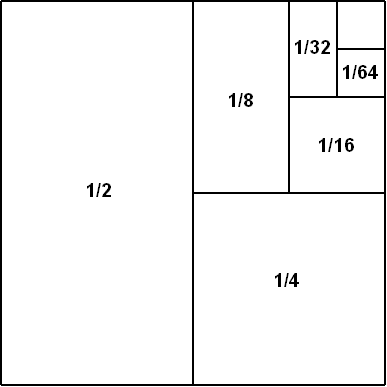
\includegraphics[scale=0.4]{img/Eye_of_Horus_square.png}
    \end{center}
    
    \item So, the number of operations is: 
    \[f(n) = 2n\]

    \item Taking out the constant, we have: 
    \[f(n) = n\]
    So, this algorithm runs in $O(n)$ time. 
\end{itemize}

\textbf{Remark:} It's important to not jump straight to conclusions. Most people (when they saw this algorithm) would have assumed an $O(n^2)$ or $O(n\log(n)$ algorithm.

\newpage 
\subsection{Common Big-O Time Complexity}
It's good to know of some Big-$O$ time complexities.
\begin{center}
    \begin{tabular}{c|c|p{7cm}}
        Big-$O$ & Common Name & Notes \\ 
        \hline 
        $O(1)$ & Constant & The time complexity does not depend on the input size $n$. \\ 
        $O(\log n)$ & Logarithmic & If the input size is doubled, the number of operations is increased by a constant. One common example is binary search: if we have 8 elements, it would take 3 operations. Doubling the number of elements would result in 4 operations. Also, it does not matter what base the logarithmic function is. \\ 
        $O(n)$ & Linear & Your algorithm scales with the number of elements linearly. For example, twice as many elements roughly means twice as slow. \\ 
        $O(n \log n)$ & & \\ 
        $O(n^2)$ & Quadratic & If the input size is doubled, we'll have quadruple the amount of elements. \\ 
        $O(n^3)$ & Cubic & Similarly to quadratic or linear, if the input size is doubled, the number of operations are multiplied by 8. \\ 
        $O(n^a)$ & Polynomial & For some constant $a$, this is known as polynomial time. All of the Big-$O$ time complexities above are considered polynomial. Anything that is upper-bounded by $O(n^a)$ is called polynomial. \\ 
        $O(k^n)$ & Exponential & For some constant $k$. \\ 
        $O(n!)$ & Factorial &  
    \end{tabular}
\end{center}

\textbf{Remark:} Anything algorithm that runs in polynomial time is considered ``good.'' Exponential and factorial time complexities are considered ``bad.''

\subsection{Space Complexity}
We can also describes algorithms by space complexity -- how much space does an algorithm need for some input size $n$? Just like time complexity, we often use Big-$O$ notation.

\bigskip 

Consider a singly linked list: 
\begin{verbatim}
    |------|     |------|     |------|     |------| 
    | Head | --> |      | --> |      | <-- | Tail | 
    |------|     |------|     |------|     |------|
\end{verbatim}
Suppose it takes $k$ bytes to store a node. If we have $n$ nodes, it would take roughly $k \cdot n$ bytes to represent all of these nodes. We will always have one head and one tail nodes (regardless of how many inputs we have), so these remain constant. Thus, the space complexity for a singly linked list is: 
\[f(n) = kn + 2c\]
Where: 
\begin{itemize}
    \item $c$ is a constant that represents the number of bytes needed to store the head and tail pointer.
    \item $k$ is a constant that represents the number of bytes needed to store a node. 
\end{itemize}

\section{Trees}
Before we can talk about trees, we need to talk about graphs. 

\subsection{Graphs}
A graph is a collection of nodes and edges. For instance, here is a simple graph: 
\begin{verbatim}
           |---|
           | B |
           |---|
          /     \
         /       \
    |---|         |---|
    | A |         | C |
    |---|         |---|
\end{verbatim}
We have nodes $A$, $B$, and $C$, that have some connection to each other. We also have edges, or links, that connect their nodes. 

\bigskip 

There are two types of edges. 
\begin{itemize}
    \item A directed edge, where we can go from one node to another node, but not the other way around. In other words, we can think of a directed edge as an \emph{one-way street}. 
    \begin{verbatim}
        |---|         |---|
        | A | ------> | B |
        |---|         |---|
    \end{verbatim}

    \item An undirected edge, where we can go from one node to another node and vice versa. In other words, we can think of an undirected edge as a \emph{two-way street}. 
    \begin{verbatim}
        |---|         |---|
        | A | ------- | B |
        |---|         |---|
    \end{verbatim}
\end{itemize}

With that said, we should observe that the simple graph that we drew above (containing nodes $A$, $B$, and $C$) could represent a linked list. In particular: 
\begin{itemize}
    \item If the edges were undirected, we would have a doubly linked list. 
    \item If the edges were directed (directional), we would have a singly linked list. 
\end{itemize}
So, a linked list is essentially a chain of nodes in sequence. We have $n$ nodes and $n - 1$ edges. 

\subsection{What are Trees?}
A tree is a graph with two properties: 
\begin{itemize}
    \item \underline{It has no undirected cycles.}
    
    \bigskip 

    In graphs, we could theoretically have something like: 
    \begin{verbatim}
               |---|
               | B |
               |---|
              /     \
             /       \
        |---|         |---|
        | A |---------| C |
        |---|         |---|
    \end{verbatim}
    This is known as a \textbf{cycle} (specifically, an undirected cycle). Essentially, we can go from $A$ to $B$, $B$ to $C$, and then back to $A$ from $C$.
    
    \bigskip 

    We can also have something like this: 
    \begin{center}
        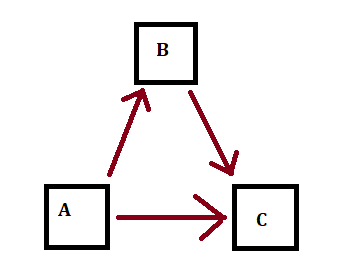
\includegraphics[scale=0.5]{img/graph_dir_cycle.PNG}
    \end{center}
    This is not a cycle because we cannot start at $A$ and end up back at $A$ (and the same applies with $B$). This is because we'll always end up stuck at $C$. And, if we start at $C$, we're stuck at $C$. That being said, if we converted each of the directed edges of this graph into undirected edges, we get an undirected cycle which is not allowed. 

    \item \underline{The nodes must be connected.} 
    
    \bigskip 

    Consider the following graph: 
    \begin{verbatim}
                    10 
                   /  \
                  /    \
                 5     15
                / \    / \
               3   7  13  20
    \end{verbatim}
    This is a graph; it has nodes and it has edges. There are no undirected cycles. Finally, all the nodes are connected (all nodes are connected to the other nodes in this tree in some way). Therefore, this is a tree. 

    \bigskip 

    Consider the following graph:
    \begin{verbatim}
        A ---- B

        C ---- D
    \end{verbatim}
    This is not a tree because nodes $A$ and $B$ are not connected to $C$ and $D$. 
\end{itemize}

\subsection{Special Cases of Valid Trees}
There are a few cases of valid trees that we should discuss. 

\begin{itemize}
    \item The empty (``null'') tree. This tree has 0 nodes and 0 edges. 

    \item A tree containing a single node. This has 1 node and 0 edges. 
    \begin{verbatim}
                |----|
                | 42 |
                |----|
    \end{verbatim}
\end{itemize}

\subsection{Rooted vs. Unrooted Trees}
Now, we talk briefly about rooted vs. unrooted trees. 

\begin{itemize}
    \item A \textbf{rooted} tree is a tree with a hierarchical structure (there is some sense of direction from top to bottom). This looks something like:  
    \begin{verbatim}
                    1
                   /|\
                  / | \
                 2  3  4 
                      / \
                     /   \ 
                    5     6
    \end{verbatim}
    With a rooted tree, we can consider some definitions. 
    \begin{itemize}
        \item For some node, the \textbf{parent} of a node is the node that is directly connected above said node. 
        \item For some node, the \textbf{child} (or \textbf{children}) of a node is/are the node(s) that are directly connected below said node.
        \item The \textbf{root} node is the node at the very top (and thus doesn't have a parent node). In the example above, node 1 is the root node.  
        \item A node is considered to be a \textbf{leaf} node if it doesn't have any children. Nodes 2, 3, 5, 6 are considered leaves.
        \item A node is considered to be an \textbf{internal} node if it does have children. Nodes 1, 4 are considered internal nodes.  
    \end{itemize}
    For example, consider node 4. This node's parent is node 1. This node has two children: node 5 and node 6. 


    \item An \textbf{unrooted} tree is one where there is not a top-to-bottom hierarchical structure, but more of an inside-outward structure. This looks something like: 
    \begin{verbatim}
        2              6
         \            /
          \          /
           1 ------ 4
          /          \ 
         /            \ 
        3              5
    \end{verbatim}
    With an unrooted tree, we now have the following definitions:
    \begin{itemize}
        \item The \textbf{neighbors} of a node are nodes that are directly connected to said node. For example, node 1 has three neighbor (2, 3, 4). Node 4 also has three neighbor (1, 5, 6).
        \item A node is considered to be a \textbf{leaf} node if it has one neighbor. 
        \item A node is considered to be an \textbf{internal} node if it has more than one neighbor. 
    \end{itemize}
\end{itemize}

\subsection{Rooted Binary Trees}
There are a lot of data structures that involve rooted binary trees. So, let's talk about them. 

\bigskip 

First and foremost, it's rooted (hence the name). This means: 
\begin{itemize}
    \item There is a root node. 
    \item All of the edges have a downward hierarchical relationship. 
\end{itemize}
Trees, in general, do not need to be binary. Any internal node can have any arbitrary number of children. \emph{However}, for a \textbf{binary tree}, any node must have either \underline{0, 1, or 2 child/children nodes}. 

\bigskip 

To emphasize this point, consider the binary tree: 
\begin{verbatim}
                    1
                   / \  
                  /   \
                 2     3 
                      / \
                     /   \ 
                    4     5
\end{verbatim}
Here, we see that: 
\begin{itemize}
    \item Nodes 2, 4, 5 have 0 children. 
    \item Node 1 has 2 children. 
    \item Node 3 has 2 children. 
\end{itemize}
This is a perfect binary tree because every node that's internal has exactly 2 children and every leaf node has exactly 0 children. \emph{However}, a binary tree can support single-child relationships. For example, let's consider the same binary tree, with an additional node: 
\begin{verbatim}
                1
               / \  
              /   \
             2     3 
            /     / \
           /     /   \ 
          6     4     5
\end{verbatim}
Here, we see that: 
\begin{itemize}
    \item Nodes 4, 5, 6 have 0 children. 
    \item Node 1 has 2 children. 
    \item Node 3 has 2 children. 
    \item Node 2 has 1 child. 
\end{itemize}
And this is still a valid binary tree (even though \code{2} only has one child.)

\subsection{Tree Traversals}
If we store our data in some tree data structure, we need a tree traversal algorithm in order to iterate through all nodes (and our data). In this class, we'll talk about the following tree traversal algorithms: 
\begin{itemize}
    \item \textbf{Preorder:} \underline{V}isit, \underline{L}eft, \underline{R}ight. 
    \item \textbf{In-Order:} Left, Visit, Right. 
    \item \textbf{Postorder:} Left, Right, Visit. 
    \item \textbf{Level-Order:} 1st Level (Left to Right), 2nd Level (Left to Right), \dots
\end{itemize} 
We should note that preorder, in-order, and postorder traversals are examples of \textbf{depth first search} (DFS) whereas level-order traversal is an example of \textbf{breadth first search} (BFS). Regardless of the tree traversal algorithm we use, we will always start at the root. 

\subsubsection{Preorder Traversal (V, L, R)}
Consider the following tree: 
\begin{verbatim}
                    0
                   / \
                  /   \
                 /     \
                1       2 
               / \     / \ 
              /   \   5   6
             3     4   \   \ 
            /           \   9
           7             8
\end{verbatim}
In a preorder traversal, we are guaranteed that for any given node, its ancestors were visited before the node itself. So, in the tree above, if we visit node 1, then we are guaranteed that node 0, its parent, has already been visited. If we visit node 3, then we are guaranteed that node 1 and node 0 have already been visited.

\bigskip 

Preorder traversal has three steps: 
\begin{itemize}
    \item Visit the current node. 
    \item Recurse to the left node. 
    \item Recurse to the right node. 
\end{itemize}

Going back to the example tree, let's run through the preorder traversal algorithm. Note that, in the tree, I'll denote \code{[n]} as saying that we are at node $n$ and \code{(n)} as saying that we have already visited node $n$. 

\begin{itemize}
    \item We start at the root node (0). 
    \begin{verbatim}
                   [0]
                   / \
                  /   \
                 /     \
                1       2 
               / \     / \ 
              /   \   5   6
             3     4   \   \ 
            /           \   9
           7             8

        Result: 0
    \end{verbatim}

    \item Now, we traverse to the left node (1).
    \begin{verbatim}
                   (0)
                   / \
                  /   \
                 /     \
               [1]      2 
               / \     / \ 
              /   \   5   6
             3     4   \   \ 
            /           \   9
           7             8

        Result: 0, 1
    \end{verbatim}

    \item Now, we traverse to the left node (3).
    \begin{verbatim}
                   (0)
                   / \
                  /   \
                 /     \
               (1)      2 
               / \     / \ 
              /   \   5   6
            [3]    4   \   \ 
            /           \   9
           7             8

        Result: 0, 1, 3
    \end{verbatim}

    \item Now, we traverse to the left node (7).
    \begin{verbatim}
                   (0)
                   / \
                  /   \
                 /     \
               (1)      2 
               / \     / \ 
              /   \   5   6
            (3)    4   \   \ 
            /           \   9
          [7]           [8]

        Result: 0, 1, 3, 7
    \end{verbatim}

    \item Now, we would traverse to the left node. However, there's nothing there! So, we're done traversing left. Here, we can try traversing right. However, once again, there is nothing to traverse to. So, we're done with node 7. Let's move back to node 3. 
    \begin{verbatim}
                   (0)
                   / \
                  /   \
                 /     \
               (1)      2 
               / \     / \ 
              /   \   5   6
           [(3)]   4   \   \ 
            /           \   9
          (7)           [8]

        Result: 0, 1, 3, 7
    \end{verbatim}

    \item Now that we're back at node 3, let's try traversing right. However, there is no right node. So, we're done with 3 and we move back up to node 1.
    \begin{verbatim}
                   (0)
                   / \
                  /   \
                 /     \
              [(1)]     2 
               / \     / \ 
              /   \   5   6
            (3)    4   \   \ 
            /           \   9
          (7)           [8]

        Result: 0, 1, 3, 7
    \end{verbatim}

    \item Now that we're back at node 1, let's try traversing right. In this case, we are able to, so we traverse to the right node (4).
    \begin{verbatim}
                   (0)
                   / \
                  /   \
                 /     \
               (1)      2 
               / \     / \ 
              /   \   5   6
            (3)   [4]  \   \ 
            /           \   9
          (7)           [8]

        Result: 0, 1, 3, 7, 4
    \end{verbatim}

    \item At node 4, there is no left or right node. So, we're done with node 4. and we can move back up to node 1. Since we've already visited node 1 and its children, we can move back up to the root node, node 0. 
    \begin{verbatim}
                  [(0)]
                   / \
                  /   \
                 /     \
               (1)      2 
               / \     / \ 
              /   \   5   6
            (3)   (4)  \   \ 
            /           \   9
          (7)           [8]

        Result: 0, 1, 3, 7, 4
    \end{verbatim}

    \item Now that we're at node 0, we can try to traverse right (since that's the only operation we can do). Since there are right nodes, we traverse to the right node (2). 
    \begin{verbatim}
                   (0)
                   / \
                  /   \
                 /     \
               (1)     [2] 
               / \     / \ 
              /   \   5   6
            (3)   (4)  \   \ 
            /           \   9
          (7)            8

        Result: 0, 1, 3, 7, 4, 2
    \end{verbatim}

    \item Node 2 has a left and right child. Of course, we're going to traverse to the left node (5). 
    \begin{verbatim}
                   (0)
                   / \
                  /   \
                 /     \
               (1)     (2)
               / \     / \ 
              /   \  [5]  6
            (3)   (4)  \   \ 
            /           \   9
          (7)            8

        Result: 0, 1, 3, 7, 4, 2, 5
    \end{verbatim}

    \item Node 5 does not have a left child, but node 5 does have a right child, so we traverse to the right node (8). 
    \begin{verbatim}
                   (0)
                   / \
                  /   \
                 /     \
               (1)     (2)
               / \     / \ 
              /   \  (5)  6
            (3)   (4)  \   \ 
            /           \   9
          (7)           [8]

        Result: 0, 1, 3, 7, 4, 2, 5, 8
    \end{verbatim}

    \item At node 8, we cannot traverse left or right. So, we're done and we traverse back to node 5; since we've done all operations possible on node 5 (we visited it, we tried to traverse left, and we tried to traverse right), we go back to node 2. 
    \begin{verbatim}
                   (0)
                   / \
                  /   \
                 /     \
               (1)    [(2)]
               / \     / \ 
              /   \  (5)  6
            (3)   (4)  \   \ 
            /           \   9
          (7)            8

        Result: 0, 1, 3, 7, 4, 2, 5, 8
    \end{verbatim}

    \item At node 2, we can only traverse to the right node. Since node 2 has a right child, we can traverse to the right node (6).
    \begin{verbatim}
                   (0)
                   / \
                  /   \
                 /     \
               (1)     (2)
               / \     / \ 
              /   \  (5) [6]
            (3)   (4)  \   \ 
            /           \   9
          (7)            8

        Result: 0, 1, 3, 7, 4, 2, 5, 8, 6
    \end{verbatim}

    \item At node 6, we cannot traverse to the left node since there is no left child. But, there is a right child so we traverse to the right node (9). 
    \begin{verbatim}
                   (0)
                   / \
                  /   \
                 /     \
               (1)     (2)
               / \     / \ 
              /   \  (5) (6)
            (3)   (4)  \   \ 
            /           \  [9]
          (7)            8

        Result: 0, 1, 3, 7, 4, 2, 5, 8, 6, 9
    \end{verbatim}

    \item At this point, we traverse back to node 6. Since we're done with node 6, we traverse back to node 2. Since we're done with node 2, we traverse back to node 0 (root node). Since we're done with node 0, we're done! Our final result is: 
    \begin{verbatim}
        0, 1, 3, 7, 4, 2, 5, 8, 6, 9
    \end{verbatim}
\end{itemize}

\subsubsection{In-order Traversal (L, V, R)}
This algorithm works like so: 
\begin{itemize}
    \item Traverse down the left subtree. 
    \item Once that's done, visit the current node. 
    \item Then traverse down the right subtree.
\end{itemize}

Unlike the other traversal algorithms, an in-order traversal only really makes sense in the context of a binary tree. \textbf{Note that}, in the tree, I'll denote \code{[n]} as saying that we are at node $n$ and \code{(n)} as saying that we \emph{have been} at node $n$ (but not necessarily visited it yet). 

\bigskip 

Consider the same tree example from the previous example. 
\begin{itemize}
    \item We start at node 0, the root node.
    \begin{verbatim}
                   [0]
                   / \
                  /   \
                 /     \
                1       2 
               / \     / \ 
              /   \   5   6
             3     4   \   \ 
            /           \   9
           7             8

        Result: 
    \end{verbatim}

    \item Because of in-order traversal, we immediately traverse to the left node. In this case, we go to node 1.  
    \begin{verbatim}
                   (0)
                   / \
                  /   \
                 /     \
               [1]      2 
               / \     / \ 
              /   \   5   6
             3     4   \   \ 
            /           \   9
           7             8

        Result: 
    \end{verbatim}

    \item Once again, we go to the left node. For the sake of saving space, we're going to condense two steps into one. First, we traverse node 3, and then we traverse node 7. 
    \begin{verbatim}
                   (0)
                   / \
                  /   \
                 /     \
               (1)      2 
               / \     / \ 
              /   \   5   6
            (3)    4   \   \ 
            /           \   9
          [7]            8

        Result: 
    \end{verbatim}

    \item We see that node 7 doesn't have a left child node! So, we \emph{visit} this node. 
    \begin{verbatim}
                   (0)
                   / \
                  /   \
                 /     \
               (1)      2 
               / \     / \ 
              /   \   5   6
            (3)    4   \   \ 
            /           \   9
          [7]            8

        Result: 7 
    \end{verbatim}

    Afterwards, we attempt to traverse to the right child node. However, there is no right child node associated with node 7, so we go back to the previous node (since we're done processing node 7).
    \begin{verbatim}
                   (0)
                   / \
                  /   \
                 /     \
               (1)      2 
               / \     / \ 
              /   \   5   6
            [3]    4   \   \ 
            /           \   9
          (7)            8

        Result: 7 
    \end{verbatim}


    \item Now that we're back at node 3, we can formally \emph{visit} it (since we're done going to the left child node). 
    
    \begin{verbatim}
                   (0)
                   / \
                  /   \
                 /     \
               (1)      2 
               / \     / \ 
              /   \   5   6
            [3]    4   \   \ 
            /           \   9
          (7)            8

        Result: 7, 3 
    \end{verbatim}

    After this, we can go back to the previous node: node 1.
    \begin{verbatim}
                   (0)
                   / \
                  /   \
                 /     \
              [(1)]     2 
               / \     / \ 
              /   \   5   6
            (3)    4   \   \ 
            /           \   9
          (7)            8

        Result: 7, 3 
    \end{verbatim}

    \item Since we've already visited node 1's left child node, we can now visit node 1 itself. 
    \begin{verbatim}
                   (0)
                   / \
                  /   \
                 /     \
              [(1)]     2 
               / \     / \ 
              /   \   5   6
            (3)    4   \   \ 
            /           \   9
          (7)            8

        Result: 7, 3, 1 
    \end{verbatim}
    Now, we attempt to traverse to node 1's right child node. Because node 1 \emph{does} have a right child node, we can traverse to it, and so we traverse to node 4. 
    \begin{verbatim}
                   (0)
                   / \
                  /   \
                 /     \
               (1)      2 
               / \     / \ 
              /   \   5   6
            (3)   [4]  \   \ 
            /           \   9
          (7)            8

        Result: 7, 3, 1 
    \end{verbatim}

    \item From node 4, we try to traverse to this node's left child. However, node 4 doesn't have a left child. So, we can actually visit node 4. 
    \begin{verbatim}
                   (0)
                   / \
                  /   \
                 /     \
               (1)      2 
               / \     / \ 
              /   \   5   6
            (3)   [4]  \   \ 
            /           \   9
          (7)            8

        Result: 7, 3, 1, 4 
    \end{verbatim}
    Once we visit node 4, we try to traverse to this node's right child. Again, this node doesn't have a right child, so we traverse back to the parent node. 
    \begin{verbatim}
                   (0)
                   / \
                  /   \
                 /     \
              [(1)]     2 
               / \     / \ 
              /   \   5   6
            (3)   (4)  \   \ 
            /           \   9
          (7)            8

        Result: 7, 3, 1, 4
    \end{verbatim}

    \item We're back at node 1, expect there's nothing to do at node 1 (since we're done with all possible operations). So, we go back to node 0 (the root node). 
    \begin{verbatim}
                  [(0)]
                   / \
                  /   \
                 /     \
               (1)      2 
               / \     / \ 
              /   \   5   6
            (3)   (4)  \   \ 
            /           \   9
          (7)            8

        Result: 7, 3, 1, 4
    \end{verbatim}

    Because we're done visiting the left child of the root node, we can now visit the node itself. 
    \begin{verbatim}
                  [(0)]
                   / \
                  /   \
                 /     \
               (1)      2 
               / \     / \ 
              /   \   5   6
            (3)   (4)  \   \ 
            /           \   9
          (7)            8

        Result: 7, 3, 1, 4, 0
    \end{verbatim}
    At this point, we can traverse to the root node's right neighbor. 
    \begin{verbatim}
                   (0)
                   / \
                  /   \
                 /     \
               (1)     [2] 
               / \     / \ 
              /   \   5   6
            (3)   (4)  \   \ 
            /           \   9
          (7)            8

        Result: 7, 3, 1, 4, 0
    \end{verbatim}

    \item For the sake of conciseness, I'll omit the remaining steps. However, the result of in-order traversal is: 
    \begin{verbatim}
        Result: 7, 3, 1, 4, 0, 5, 8, 2, 6, 9
    \end{verbatim}
\end{itemize}

\subsubsection{Postorder Traversal (L, R, V)}
In postorder traversal, I'm guaranteed that, before I visit any of a node, that I have visited that node's descendents. The idea is as follows:
\begin{itemize}
    \item Start by visiting the left nodes. 
    \item Then, visit the right nodes. 
    \item After those nodes are all visited, then visit the current
\end{itemize}

As usual, we're going to stick with the binary tree that we've used. \textbf{Note that}, in the tree, I'll denote \code{[n]} as saying that we are at node $n$ and \code{(n)} as saying that we \emph{have been} at node $n$ (but not necessarily visited it yet). 

\begin{itemize}
    \item Begin at the root node as always. 
    \begin{verbatim}
                   [0]
                   / \
                  /   \
                 /     \
                1       2 
               / \     / \ 
              /   \   5   6
             3     4   \   \ 
            /           \   9
           7             8

        Result: 
    \end{verbatim}

    \item Let's now traverse to node 1, or node 0's left child node.
    \begin{verbatim}
                   (0)
                   / \
                  /   \
                 /     \
               [1]      2 
               / \     / \ 
              /   \   5   6
             3     4   \   \ 
            /           \   9
           7             8

        Result: 
    \end{verbatim}

    \item From node 1, we can traverse to node 3 and then node 7.
    \begin{verbatim}
                   (0)
                   / \
                  /   \
                 /     \
               (1)      2 
               / \     / \ 
              /   \   5   6
            (3)    4   \   \ 
            /           \   9
           [7]           8

        Result: 
    \end{verbatim}

    At this point, since node 7 doesn't have any child nodes, we cannot traverse to node 7's left or right child nodes. Therefore, we can visit node 7. 
    \begin{verbatim}
                   (0)
                   / \
                  /   \
                 /     \
               (1)      2 
               / \     / \ 
              /   \   5   6
            (3)    4   \   \ 
            /           \   9
           [7]           8

        Result: 7
    \end{verbatim}

    \item Now, we can traverse back to node 3.
    \begin{verbatim}
                   (0)
                   / \
                  /   \
                 /     \
               (1)      2 
               / \     / \ 
              /   \   5   6
           [(3)]   4   \   \ 
            /           \   9
           (7)           8

        Result: 7
    \end{verbatim}
    At node 3, we've already traversed to the left child node (7). Since node 3 doesn't have a right child node, we cannot traverse to that node. Therefore, we can visit node 3:
    \begin{verbatim}
                   (0)
                   / \
                  /   \
                 /     \
               (1)      2 
               / \     / \ 
              /   \   5   6
           [(3)]   4   \   \ 
            /           \   9
           (7)           8

        Result: 7, 3
    \end{verbatim}

    \item Now, we can traverse to node 1. 
    \begin{verbatim}
                   (0)
                   / \
                  /   \
                 /     \
              [(1)]     2 
               / \     / \ 
              /   \   5   6
            (3)    4   \   \ 
            /           \   9
           (7)           8

        Result: 7, 3
    \end{verbatim}

    At node 1, we now need to visit the right child node, so we do that. 
    \begin{verbatim}
                   (0)
                   / \
                  /   \
                 /     \
               (1)      2 
               / \     / \ 
              /   \   5   6
            (3)   [4]  \   \ 
            /           \   9
           (7)           8

        Result: 7, 3
    \end{verbatim}
    Since node 4 doesn't have a left or right child node, we cannot traverse to the left or right child node. So, we visit node 4.
    \begin{verbatim}
                   (0)
                   / \
                  /   \
                 /     \
               (1)      2 
               / \     / \ 
              /   \   5   6
            (3)   [4]  \   \ 
            /           \   9
           (7)           8

        Result: 7, 3, 4
    \end{verbatim}

    \item Now, we can traverse back to node 1. 
    \begin{verbatim}
                   (0)
                   / \
                  /   \
                 /     \
              [(1)]     2 
               / \     / \ 
              /   \   5   6
            (3)   (4)  \   \ 
            /           \   9
           (7)           8

        Result: 7, 3, 4
    \end{verbatim}
    Since we already traversed to node 1's left and right child nodes (and thus node 1's left and right subtrees), we can visit node 1.
    \begin{verbatim}
                   (0)
                   / \
                  /   \
                 /     \
              [(1)]     2 
               / \     / \ 
              /   \   5   6
            (3)   (4)  \   \ 
            /           \   9
           (7)           8

        Result: 7, 3, 4, 1
    \end{verbatim}

    \item Now, we can traverse back to node 0. 
    \begin{verbatim}
                  [(0)]
                   / \
                  /   \
                 /     \
               (1)      2 
               / \     / \ 
              /   \   5   6
            (3)   (4)  \   \ 
            /           \   9
           (7)           8

        Result: 7, 3, 4, 1
    \end{verbatim}

    Now that we're at node 0, we need to traverse to the right child node. So, we do that. 
    \begin{verbatim}
                   (0)
                   / \
                  /   \
                 /     \
               (1)     [2] 
               / \     / \ 
              /   \   5   6
            (3)   (4)  \   \ 
            /           \   9
           (7)           8

        Result: 7, 3, 4, 1
    \end{verbatim}

    \item We've now traversed to node 2. At this point, we need to traverse to node 2's left and right child nodes. To save some steps, we'll do it all in one go. Namely: 
    \begin{itemize}
        \item We traverse to node 5, and then node 8 (since node 5 doesn't have a left child node). 
        \item Because node 8 doesn't have a left or right child node, we visit node 8 and go back to node 5.
        \item Because we've visited node 5's left and right child nodes (noting that node 5 doesn't even have a left child node), we can visit node 5 and then go back to node 2. 
        \item Now that we're at node 2, we can traverse to node 6, and then back to node 9. 
        \item At node 9, there is no left or right child node so we can visit node 9 and go back to node 6. 
        \item At node 6, because there's no left child node and the right child node has already been visited, we can visit node 6 and go back to node 2. 
        \item Since we've visited all of node 2's left and right child nodes, we can visit node 2 and go back to node 0, the root node. 
        \item Since we've visited all of node 0's left and right child nodes, we can visit node 0. Thus, we're done.
    \end{itemize}

    \item The final result, then, is: 
    \begin{verbatim}
        Result: 7, 3, 4, 1, 8, 5, 9, 6, 2, 0
    \end{verbatim}
\end{itemize}

\subsubsection{Level-Order Traversal}
Unlike the other three algorithm, level-order traversal is an example of breadth first search. 

\bigskip 

The idea is relatively simple. We're traversing with respect to distance away from the root. In this sense, we're traversing like so: 
\begin{verbatim}
                    0               -------->
                   / \
                  /   \
                 /     \
                1       2           -------->
               / \     / \ 
              3   4   5   6         -------->
             /         \   \ 
            7           8   9       -------->
\end{verbatim}
So, essentially, if we traversed using level-order traversal, our result would be: 
\begin{verbatim}
    Result: 0, 1, 2, 3, 4, 5, 6, 7, 8, 9
\end{verbatim}


\section{Binary Search Trees}
A binary search tree is a special type of binary tree with the following properties: 
\begin{itemize}
    \item It must be a rooted binary tree (can only have 0, 1, or 2 children). 
    \item Every node is larger than all nodes in its left subtree. 
    \item Every node is smaller than all nodes in its right subtree. 
\end{itemize}

Consider the following tree: 
\begin{verbatim}
            10
           /  \  
          /    \ 
         /      \ 
        5       15 
       / \        \ 
      /   \        \ 
     2     7       20 
                   /
                  17 
\end{verbatim}
This is a valid binary search tree because: 
\begin{itemize}
    \item It's rooted. 
    \item Each node has 0, 1, or 2 children. 
    \item For any given node, its left node's value are smaller than the given node's value. For example, for node 5, $2 < 5$. Another example is for node 10, where $2 < 5 < 7 < 10$. 
    \item For any given node, its right node's values are bigger than the given node's value. For example, for node 5, $5 < 7$. Another example is for node 10, where $10 < 15 < 17 < 20$.
\end{itemize}

Consider the following tree: 
\begin{verbatim}
            10 
           /  \  
          5    20
              /  \  
             9    30
\end{verbatim}
This is not a binary search tree. While node 20's left and right child nodes meet the criteria ($9 < 20$ and $20 < 30$), node 9 is on the right of node 10 and we know that $10 < 9$ is false. 

\subsection{BST Find Algorithm}
Denote \code{query} to be the query (the element we want to find) and \code{current} to be the current node (the node that we're at). The binary search tree find algorithm works as follows
\begin{enumerate}
    \item Start at the root. 
    \item If \code{query == current}, success! 
    \item Otherwise, if \code{query > current}, traverse right and go back to step 2. 
    \item Otherwise, if \code{query < current}, traverse left and go back to step 2. 
\end{enumerate}
\textbf{Remark:} If we try to traverse left or right but no such child exists, then the element doesn't exist. 

\bigskip 

Consider the following BST: 
\begin{verbatim}
            50 
           / \
          /   \
         20    70 
        /  \    \ 
       10  25   100 
\end{verbatim}
Let's suppose we tried to look for \code{20} (so \code{query = 20}). We start at node 50 (so \code{current = 50}). 
\begin{itemize}
    \item Since \code{current = (50 != 20) = query}, we need to check the child nodes. 
    \item Since \code{query = (20 < 50) = current}, we traverse to the left child. Thus, \code{current = 20}.
    \item Since \code{current = (20 == 20) = query}, we're done. 
\end{itemize}

Let's now suppose we tried to look for \code{25}. Once again, \code{query = 25} and \code{current = 50}.
\begin{itemize}
    \item Since \code{current = (50 != 25) = query}, we need to check the child nodes. 
    \item Since \code{query = (25 < 50) = current}, we traverse to the left child. Thus, \code{current = 20}.
    \item Since \code{current = (20 != 25) = query}, we need to check the child nodes.
    \item Since \code{query = (25 > 20) = current}, we need to check the right child. Thus, \code{current = 25}.
    \item Since \code{current = (25 == 25) = query}, we're done. 
\end{itemize}

Finally, let's suppose we tried to find \code{60}. Once again, \code{query = 60} and \code{current = 50}. 
\begin{itemize}
    \item Since \code{current = (50 != 60) = query}, we need to check the child nodes. 
    \item Since \code{query = (60 > 50) = current}, we go to the right child. Thus, \code{current = 70}.
    \item Since \code{current = (70 != 60) = query}, we need to check the child nodes.
    \item Since \code{query = (60 < 70) = current}, we go to the left child. Since 70 does not have a left child, the element is not found. 
\end{itemize}

\subsection{BST Insert Algorithm}
The binary search tree insert algorithm works as follows
\begin{enumerate}
    \item Perform \code{find} operation, starting at the root. 
    \item If \code{find} succeeds, there is a duplicate element so we don't insert. 
    \item If \code{find} doesn't succeed, insert the new element at the site of failure. 
\end{enumerate}

Let's consider a very simple binary search tree: 
\begin{verbatim}
            50 
              \ 
              70 
                \ 
                100 
\end{verbatim}

Let's suppose we tried to insert \code{100}. Since \code{100} exists in the binary search tree, we don't need to add this element. 

\bigskip 

Let's suppose we tried to insert \code{65}. Since \code{65} does not exist in the binary search tree, we can add it to the binary search tree. To be concrete: 
\begin{itemize}
    \item We start at \code{50} (root element). 
    \item Since \code{current != 65} but \code{current < 65}, we traverse to the right child. Now, \code{current = 70}. 
    \item Since \code{current != 65} but \code{current > 65}, we traverse to the left child.
    \item Since there is nothing to traverse to (node 70 doesn't havea  left child), we append \code{65}, like so:
    \begin{verbatim}
            50 
              \ 
              70 
             /  \ 
            65  100 
    \end{verbatim}
\end{itemize}

As a final example, suppose we tried to insert \code{67}. The algorithm will run like so: 
\begin{itemize}
    \item We start at \code{50} (root). 
    \item Since \code{current != 67} but \code{current < 67}, we traverse to the right child. Now, \code{current = 70}. 
    \item Since \code{current != 67} but \code{current > 67}, we traverse to the left child. So, \code{current = 65}.
    \item Since \code{current != 65}, but \code{current < 67}, we traverse to the right child. 
    \item But, since there's nothing to traverse to (node 65 doesn't have a right child), we append \code{67} like so: 
        \begin{verbatim}
            50 
              \ 
              70 
             /  \ 
            65  100
             \
             67 
    \end{verbatim}
\end{itemize}

\subsection{BST Successor Algorithm}
What is a node successor? Given some node $U$, the successor of node $U$ is the next largest node. In other words, it's the node that is immediately larger than node $U$. 

\bigskip 

Consider the following binary search tree\footnote{The tree is a bit oversized due to the way text is formatted, don't worry about that.}: 
\begin{verbatim}
                               E
                    __________/ \__________
                   /                       \ 
                  /                         \
                 /                           \ 
                B                             H
               / \                           / \
              /   \                         /   \ 
             /     \                       /     \
            A       C                     G       I
                     \                   / 
                      \                 /
                       \               /
                        D             F
\end{verbatim}
The successors are as follows: 
\begin{itemize}
    \item The successor of $A$ is $B$. 
    \item The successor of $B$ is $C$. 
    \item The successor of $C$ is $D$. 
    \item The successor of $D$ is $E$. 
    \item The successor of $E$ is $F$.
    \item The successor of $F$ is $G$. 
    \item The successor of $G$ is $H$. 
    \item The successor of $H$ is $I$.  
\end{itemize}

If we had an efficient algorithm to determine the successor of a node, then we can implement an efficient iterator that would iterate over our binary search tree in increasing order of size.

\bigskip 

How do we find the successor of a given node? The algorithm is as follows: 
\begin{itemize}
    \item If the node has a right child, traverse right once, then all the way left. 
    
    \bigskip 

    Consider the following examples: 
    \begin{itemize}
        \item If we wanted to find the successor of $E$, we would traverse right once ($E \to \boxed{H}$) and then traverse all the way left ($H \to G \to \boxed{F}$).
        \item If we wanted to find the successor of $B$, we would traverse right once ($B \to C$) and then traverse all the way left. Since $C$ doesn't have any left child nodes, $\boxed{C}$ is the successor. 
    \end{itemize}

    \item Otherwise, traverse up the tree. The first time the current node is its parent's left child, the parent is our successor. 
    
    \bigskip 

    Consider the following examples: 
    \begin{itemize}
        \item Suppose we wanted to find the successor of $D$. We note that $D$ doesn't have a right child, so we cannot do the first step of this algorithm and must go to this step of the algorithm. 
        \begin{itemize}
            \item First, we note that $D$ is $C$'s \emph{right} child. So, the left child condition isn't met. So, we go up one. 
            \item We note that $C$ is $B$'s right child again, so the left child condition isn't met. 
            \item We note that $B$ is $E$'s \emph{left} child. So, the left child condition is met. Therefore, $E$ is the successor of $D$. 
        \end{itemize}

        \item Suppose we wanted to find the successor of $A$. We note that $A$ doesn't have a right child, so we need to do this step of the algorithm.
        \begin{itemize}
            \item First, we note that $A$ is $B$'s left child. So, the left child condition is met; thus, $B$ is the successor of $A$. 
        \end{itemize}
    \end{itemize}
\end{itemize}

\subsection{BST Remove Algorithm}
As usual, we begin by running the find algorithm. However, if we find the node to delete, we need to consider three cases. 

\begin{enumerate}
    \item \underline{No Children:} Just delete the node. 
    \item \underline{One Child:} Just directly connect my child to my parent. 
    \item \underline{Two Children:} Replace my value with my successor's value, and remove me. 
\end{enumerate}

\subsubsection{Case 1: No Children}
Consider the following binary search tree: 
\begin{verbatim}
        2
       / \ 
      1   3
\end{verbatim}
If we wanted to remove \code{3}, we can just delete it since it has no children. We can set the parent (\code{2})'s right child node to \code{nullptr}.
\begin{verbatim}
    2
   /  
  1   
\end{verbatim}

\subsubsection{Case 2: One Child}
Consider the following binary search tree: 
\begin{verbatim}
        2
       / \ 
      1   3 
           \ 
            4
\end{verbatim}
Suppose we wanted to remove \code{3}, we can simply link \code{2} with \code{4}, like so: 
\begin{verbatim}
    2
   / \ 
  1   4 
\end{verbatim}

\subsubsection{Case 3: Two Children}
Consider the following binary search tree: 
\begin{verbatim}
        2 
       / \ 
      /   \ 
     1     4 
          / \ 
         /   \ 
        3     5
\end{verbatim}
Suppose we wanted to remove \code{4}. To do so, we need to find node \code{4}'s successor value, put the successor's value in the node's place, and then remove the node itself. We know that node \code{4}'s successor is \code{5}, so we swap their values and then delete the node containing the value that we wanted to remove (in this case, it's the node that we swapped withthe successor). A visualization is shown below\footnote{I put \code{[]} to emphasize the two nodes being swapped. It serves no other purpose.}:
\begin{verbatim}
        2                 2                   2                   
       / \               / \                 / \                  
      /   \             /   \               /   \ 
     1    [4]   --->   1     5     --->    1     5 
          / \               / \                 / 
         /   \             /   \               /
        3    [5]          3     4             3
\end{verbatim}


But, what if we had a more complex example? Suppose we had to deal with this binary search tree: 
\begin{verbatim}
        2
       / \ 
      /   \ 
     1     4 
          / \  
         /   \ 
        3     6
               \ 
                \ 
                 7
\end{verbatim}
Suppose we wanted to remove \code{4}. \code{4}'s successor is \code{6}. We begin by swapping the two values like usual. Then, we can remove the node where \code{4} is at right now and attach the now-deleted node's child node to node \code{6}.  
\begin{verbatim}
        2                        2                        2
       / \                      / \                      / \ 
      /   \                    /   \                    /   \  
     1    [4]                 1     6                  1     6 
          / \       --->           / \        --->          / \  
         /   \                    /   \                    /   \ 
        3    [6]                 3     4                  3     7
               \                        \                         
                \                        \                         
                 7                        7
\end{verbatim}

\subsection{Height of a Node and Tree}
Consider this tree (which we'll use for some examples to supplement the definitions):
\begin{verbatim}
            5
           / \ 
          /   \ 
         /     \ 
        1       7
               / \ 
              /   \ 
             /     \ 
            6       8 
                     \ 
                      \ 
                       \ 
                        9
\end{verbatim}

Then, we say that: 
\begin{itemize}
    \item The \textbf{height} of a \textbf{node} is the \underline{longest} distance (number of edges) from said node to a leaf. 
    
    \bigskip 

    In the above tree:
    \begin{itemize}
        \item The distance from node 9 to a leaf is 0 (no edges). 
        \item The distance from node 8 to a leaf is 1 (1 edge).
        \item The distance from node 7 to a leaf is 2. Although node 7 can reach two different leaf nodes (6, 9), we are only interested in the farthest leaf node (9).
        \item The distance from node 5 to a leaf is 3. Although node 5 can reach three different leaf nodes (1, 6, 9), we are only interested in the farthest leaf node (9). 
    \end{itemize}

    \item The \textbf{height} of a \textbf{tree} is the height of the root of the tree. 
    
    \bigskip 

    The root of the tree is node 5, so we say that the height of the tree is 3 (since we want to find the distance from the root node to the farthest leaf node).
\end{itemize}

\subsection{Tree Balance}
We can think of tree balance as a metric of how tall a tree is with respect to the number of nodes it has. In particular, for some $n$, we can think of tree balancing as a spectrum between perfectly unbalanced and perfectly balanced. 

\bigskip 

Consider $n = 7$ (a tree with 7 nodes).
\begin{verbatim}
    |-------------------------------------------------------------------------------|
    Perfectly Unbalanced                                           Perfectly Balanced 

    1                                                                       4
     \                                                                     / \  
      2                                                                   /   \ 
       \                                                                 /     \ 
        3                                                               /       \ 
         \                                                             2         6 
          4                                                           / \       / \  
           \                                                         /   \     /   \  
            5                                                       1     3   5     7 
             \                                             
              6                                           
               \                                          
                7
\end{verbatim}
In a perfectly unbalanced tree, we have a height of \textbf{6}. In a perfectly balanced tree, we have a height of \textbf{2}. Both trees are binary search trees.

\bigskip 

Basically, a perfectly unbalanced binary search tree is like a linked list. 

\subsection{Time Complexity}
Part of evaluating the time complexity of any BST is figuring out the tree's shape; whether the tree is balanced or unbalanced will make a difference. 

\bigskip 

For the \code{find}, \code{insert}, and \code{delete} operations, the worst-case runtime is as follows: 
\begin{center}
    \begin{tabular}{c|c|p{7cm}}
        \textbf{Tree Type} & \textbf{Worst Case Big-$O$} & \textbf{Why?} \\
        \hline 
        Perfectly Unbalanced Tree & $\boxed{O(n)}$ & For a perfectly unbalanced tree, if we have $n$ nodes, then a perfectly unbalanced tree will have a height of $n - 1$. The worst case would occur if we had to traverse over all the edges of the tree. \\
        Perfectly Balanced Tree   & $O(\log(n))$ & The reason why this is $O(\log(n))$ -- more specifically, $O(\log_{2}(n + 1) - 1)$ -- is because even if we double the number of nodes in a tree, the tree's height would only grow by 1.
    \end{tabular}
\end{center}
\textbf{Remark:} $O(\log(n))$ is not actually the worst case; this is actually a very nice case simply because this assumes that a tree is perfectly balanced. In other words, \emph{if} the tree was perfectly balanced, the worst-case runtime would be $O(\log(n))$; however, because any given tree will probably not be perfect, we cannot make that assumption. So, the worst-case runtime for any given binary search tree is actually $O(n)$. 

\subsubsection{Find Algorithm: Best vs. Worst vs. Average Case}
We should note that: 
\begin{itemize}
    \item The \textbf{best} case scenario is if the query is the root. 
    \item The \textbf{worst} case scenario is if we need to work with a perfectly unbalanced tree and the query is not found. 
    \item The \textbf{average} case scenario is the theoretical expected value over all trees and queries. 
\end{itemize}

For $n$ elements as $n \to \infty$:
\begin{center}
    \begin{tabular}{c|c|p{7cm}}
        \textbf{Case} & \textbf{Runtime} & \textbf{Remark(s)} \\ 
        \hline 
        Best & $O(1)$ & It doesn't matter if the tree is perfectly balanced or unbalanced if the root node is the right node. \\ 
        Worst & $O(n)$ & If the tree is perfectly unbalanced and the value was either not found or is the last node in the tree (i.e. a leaf node). 
    \end{tabular}
\end{center}

The average case is a bit more complicated. In particular, we need to assume the following:
\begin{enumerate}
    \item All $n$ elements are equally likely to be searched for. 
    
    \bigskip 

    If we had a binary search tree with the elements $1, 2, 3$, then: 
    \[P(Q = 1) = P(Q = 2) = P(Q = 3) = \frac{1}{n} = \frac{1}{3}\]
    This is saying that the probability that our query is \code{1} is the same as the probability that our query is \code{2} which is the same as saying that the probability that our query is \code{3}, or $\frac{1}{3}$. This holds for $n$ elements. 

    \item All $n!$ possible insertion orders are equally likely. 
    
    \bigskip 

    If we had the elements $1, 2, 3$, there are $3! = 6$ possible insertion orders: 
    \begin{itemize}
        \item 123 
        \item 132 
        \item 213
        \item 231
        \item 312
        \item 321 
    \end{itemize}
    \emph{However}, \code{213} and \code{231} gave us the same tree structure. So, there are 5 unique tree structures for 6 possible insertion orders. 
\end{enumerate}

\subsubsection{Depth of a Node}
The \textbf{depth of a node} is the number of nodes in the path from that node to the root. 

\bigskip 

For example, consider the following binary search tree: 
\begin{verbatim}
                8 
               / \ 
              /   \ 
             /     \ 
            3      10
           / \       \ 
          /   \       \ 
         1     6      14
              / \     /
             4   7   13
\end{verbatim}
We can say that: 
\begin{itemize}
    \item The number of nodes from the root node to itself is \textbf{1}: itself. 
    \item The number of nodes from node 10 to the root node is \textbf{2}. 
    \item The number of nodes from node 14 to the root node is \textbf{14}.
    \item The number of nodes from node 13 to the root node is \textbf{4}. 
    \item The number of nodes from node 3 to the root node is \textbf{2}.
    \item The number of nodes from node 6 to the root node is \textbf{3}. 
    \item The number of nodes from node 4 to the root node is \textbf{4}. 
    \item The number of nodes from node 7 to the root node is \textbf{4}. 
    \item The number of nodes from node 1 to the root node is \textbf{3}. 
\end{itemize}
The \textbf{average case time complexity} is the \underline{expected number of operations to find a query}. 

\bigskip 

Suppose one operation is one comparison and we were looking for the number \code{3}. This would require \textbf{2} comparisons, or 2 operations. The average case time complexity is the expected number of operations for every node in this tree. This is equivalent to the \underline{expected depth}. 

\bigskip 

Generally speaking, the number of comparisons to find a node is equal to the depth of that node. 


\end{document}